\documentclass{IEEEtran}

\usepackage{listings}
\lstset{
    basicstyle=\small\ttfamily,
    breaklines=true
}
\usepackage{graphicx}
\graphicspath{ {./images/} }

\title{Readings about DP and Recursion}
\author{Diego Linares - kiwiAipom}

\begin{document}
    \maketitle

    \section{Everything about Dynamic Programming}

    \section{Some general approach for solving recursive problems}
        \textbf{Step One:} Think about any input for which you know what your function should return.\\
        Now suppose you have a task, related to a similar one. Keep calling that function to solve it: \textit{I'll solve the problem if you give me this subproblem first}. Which is done by a call to the same function.\\
        \textbf{Example:} With factorial, you only know that $0!=1$ and $n!=n(n-1)!$. So the function that gives me factorial of $n$ just needs the results of one that returns $(n-1)!$. This will keep going as long as we don't know whaat value to return.
        \begin{lstlisting}
factorial(n):
    if n = 0:
        return 1 // I know this, so I don't want my function to go any further
    else:
        return n*factorial(n-1) // just reuse the function
        \end{lstlisting}
        \textbf{Step Two:} They can do the same as loops, a simple \texttt{for} can be implemented as:
        \begin{lstlisting}
for(i, n):
    if i = n:
        return // Terminates
    // Do whatever needed
    for(i+1, n) // Next iteration
        \end{lstlisting}
        And for backwards:
        \begin{lstlisting}
rof(i, n):
    if i = n:
        return // Terminates
    rof(i+1, n) // Next iteration    
    // Do whatever needed
        \end{lstlisting}
        Since the function calls itself again until reaching a limit value and then starts returning.\\
        \textbf{Example:} To print numbers backwards you may do this:
        \begin{lstlisting}
function(i, n):
    if i <= n:
        function(i+1, n)
        print(i)
        \end{lstlisting}
        Which for numbers from 1 to 5 would work like:\\
        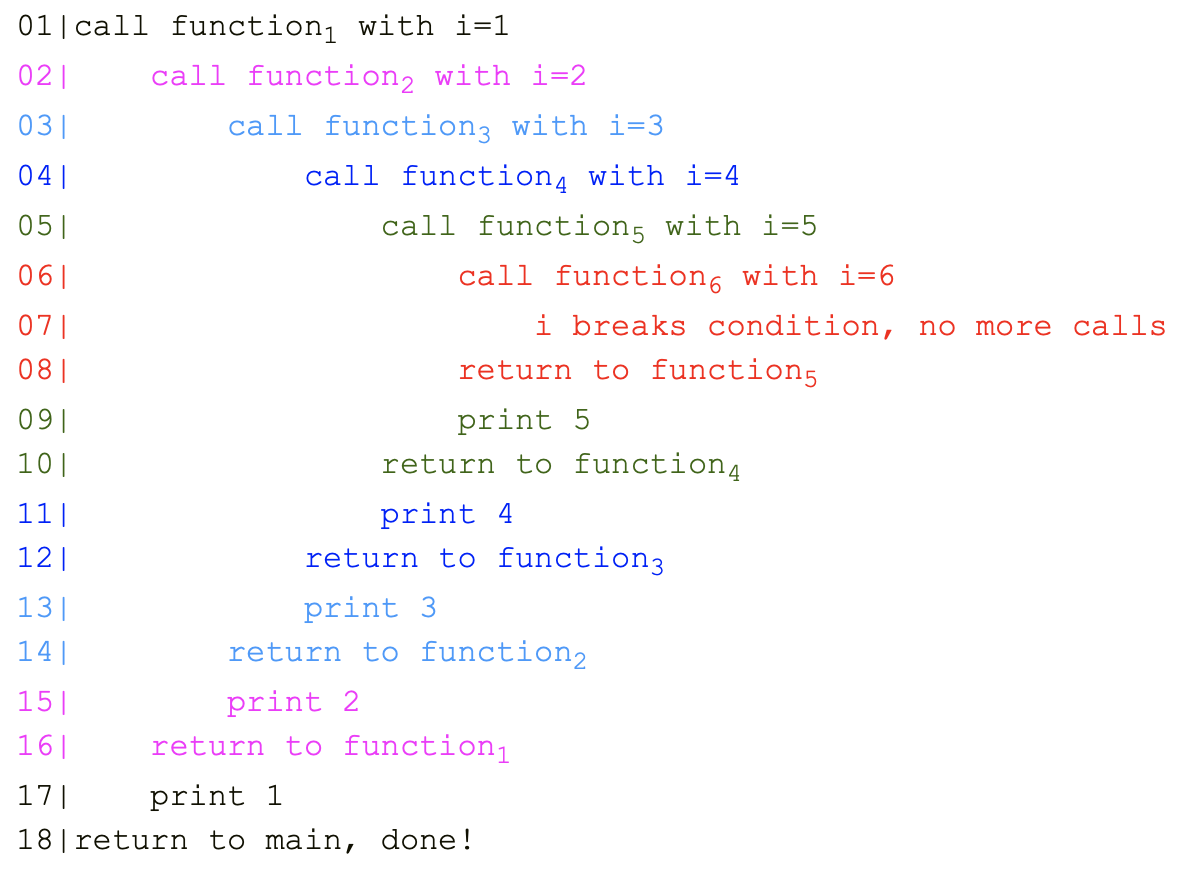
\includegraphics[width=0.4\textwidth]{rofExecution.png}\\
        \textbf{Step Three:} There's a stack call which looks like this:\\
        \begin{center}
            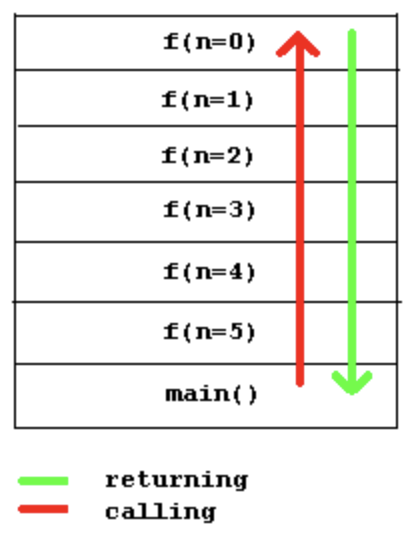
\includegraphics[width=0.15\textwidth]{stackCalls.png}
        \end{center}
        The memory of $f(3)$ for example, won't be freed until $f(2)$ is done. Serves the purpose of using an array, since the functions store variables and values.\\
        \textbf{Step Four:} Be careful, in CP they are generally avoided since most can be done iteratively, andd they may exceed time and memory. Since every function is alloted a space at the moment it is called, might run into RTE. Use only $O(\lg{n})$ and small $O(n)$ recursions. \\
        \textbf{Step Five:} When there are overlapping branches in the recursion tree we store computed values (DP).
    \section{Dynamic programming 2}

    \section{Matrix}

    \begin{thebibliography}{}
        \bibitem{mmi}
            \textit{Attacking Recursions},
            I Me and Myself.
            From: https://zobayer.blogspot.com/2009/12/cse-102-attacking-recursion.html
    \end{thebibliography}

\end{document}